\documentclass[12pt]{article}
\usepackage[utf8]{inputenc}
\usepackage[spanish,es-nodecimaldot]{babel}
\usepackage{amsmath, amssymb, amsthm}
\usepackage{graphicx}
\usepackage{float}
\usepackage{hyperref}
\usepackage{siunitx}
\usepackage{geometry}
\usepackage{svg}
\usepackage{float}
\usepackage{fancyhdr}
\geometry{a4paper, margin=1in}

\setlength{\headheight}{1pt}  
\setlength{\headsep}{55pt}  

\sisetup{group-separator = {,}}


\pagestyle{fancy}
\fancyhf{} 
\fancyhead[L]{\includegraphics[width=4cm]{images/logo-usm2.png}}
\fancyhead[R]{\textbf{MAT-043: Probabilidad y Estadística}}




\begin{document}



\begin{titlepage}
    \centering
    \vspace*{1cm}  % Espacio superior para centrar mejor

    % Logo
    \includesvg[scale=0.4]{images/logo-usm.svg}  % Ajusta el logo según la ruta de tu imagen
    \vspace{2cm}  % Espacio entre el logo y el título

    % Título
    {\LARGE \textbf{Simulaciones y Probabilidad:}} \\[0.5cm]
    {\LARGE \textbf{Un Enfoque Computacional para la Estadística Aplicada}} \\[1.5cm]

    % Información del curso
    {\Large Proyecto MAT-043: Probabilidad y Estadística} \\[0.5cm]

    % Autoría
    \vspace{1cm}
    {\large \textbf{Autores:}} \\[0.3cm]
    {\large Francisco González, Karime Jarufe} \\[1.5cm]

    % Profesor
    {\large \textbf{Profesor:}} \\[0.3cm]
    {\large Dr. Ronny O. Vallejos} \\[2.5cm]

    % Fecha
    {\large \textbf{Noviembre 25, 2024}} \\

    \vfill  % Rellena el espacio restante para centrar los elementos

    % Pie formal (opcional)
    %{\footnotesize Universidad Técnica Federico Santa María \\ Departamento de Matemática}
\end{titlepage}


\newpage
\tableofcontents
\newpage

\section{Motivación}

En un mundo cada vez más impulsado por datos, el análisis estadístico y la modelación probabilística se han convertido en herramientas fundamentales para la toma de decisiones informadas. Estas metodologías permiten abordar problemas complejos, identificar patrones, y estimar resultados bajo condiciones de incertidumbre en diversos campos como la economía, la ingeniería, la gestión operativa y las ciencias aplicadas. La probabilidad y la estadística computacional, en particular, ofrecen soluciones prácticas y precisas a problemas que desafían los enfoques tradicionales, al combinar el rigor teórico con el poder del cálculo moderno.

Este proyecto surge de la necesidad de explorar estas herramientas en escenarios reales, donde el análisis de datos y la simulación computacional se convierten en aliados indispensables para optimizar procesos, mejorar recursos y generar información valiosa. Ejemplos de estos desafíos incluyen modelar el comportamiento de mercados inmobiliarios, estimar la capacidad de atención en sistemas de transporte y hospitales, y prever escenarios operativos bajo incertidumbre.

El uso de métodos computacionales como la simulación Monte Carlo resulta especialmente relevante, ya que permite analizar situaciones en las que las soluciones analíticas son inalcanzables o extremadamente complejas. Estos enfoques ofrecen una base robusta para enfrentar problemas que requieren respuestas precisas, dinámicas y adaptables a condiciones cambiantes.

En esencia, este proyecto está motivado por el deseo de conectar el rigor teórico de la probabilidad y la estadística con aplicaciones prácticas y computacionales que resuelvan problemas reales. A través de esta unión, no solo se busca generar soluciones efectivas, sino también resaltar la importancia de la estadística computacional como una herramienta clave en la innovación, la planificación estratégica y la toma de decisiones basadas en datos.

\section{Introducción}

El presente proyecto tiene como objetivo aplicar técnicas avanzadas de probabilidad y estadística para abordar problemas prácticos en contextos diversos. Utilizando herramientas computacionales modernas y métodos como la simulación Monte Carlo, este trabajo ilustra cómo los principios teóricos de la estadística pueden implementarse y evaluarse en situaciones reales, generando soluciones tanto analíticas como simuladas.

La simulación Monte Carlo, en particular, constituye una metodología fundamental en este proyecto, ya que permite modelar sistemas complejos mediante la generación de variables aleatorias y la repetición masiva de experimentos computacionales. Este enfoque resulta invaluable cuando los métodos analíticos convencionales no son viables o cuando los resultados deben estimarse en condiciones de incertidumbre. 

A lo largo del proyecto, se abordan problemas variados que reflejan la amplitud y versatilidad de las herramientas estadísticas. Entre estos, se incluyen el análisis de precios de venta de casas en un mercado inmobiliario, la optimización de recursos en vuelos comerciales mediante el cálculo de asientos extra, y la evaluación de la capacidad operativa en un sistema hospitalario. Cada uno de estos casos combina el análisis teórico con la implementación computacional para obtener resultados relevantes y precisos.

El enfoque principal del proyecto es demostrar cómo las herramientas de probabilidad y estadística computacional no solo permiten entender fenómenos complejos, sino también ofrecer soluciones prácticas para optimizar procesos y recursos. Al aplicar estos métodos, se busca contribuir al desarrollo de sistemas más eficientes y adaptables, mostrando la relevancia de estas técnicas en la ingeniería, la ciencia aplicada y la toma de decisiones estratégicas.



\section{Metodología}
\subsection{Herramientas Utilizadas}

El presente proyecto fue desarrollado utilizando herramientas computacionales basadas en Python, aprovechando su flexibilidad para el análisis de datos, simulaciones y visualización gráfica. A continuación, se describen las principales bibliotecas y métodos teóricos empleados:

\subsubsection*{Bibliotecas Utilizadas}
\begin{itemize}
    \item \textbf{Pandas:} Permite la manipulación y análisis eficiente de datos estructurados. Fue utilizada para cargar y explorar conjuntos de datos como el \textit{Ames Housing Dataset} en el Problema 1.
    \item \textbf{NumPy:} Se empleó para cálculos numéricos avanzados, como la generación de números pseudoaleatorios provenientes de distribuciones específicas (normal, log-normal, exponencial, etc.).
    \item \textbf{Matplotlib y Seaborn:} Estas bibliotecas fueron clave para la creación de gráficos, como histogramas, boxplots y violin plots, proporcionando herramientas visuales que permiten interpretar patrones en los datos.
    \item \textbf{SciPy:} Utilizada para el ajuste de distribuciones a datos empíricos y para funciones estadísticas avanzadas, como intervalos de confianza y pruebas de bondad de ajuste.
    \item \textbf{Stats (SciPy):} Implementada para realizar análisis inferenciales, como el cálculo de intervalos de confianza en el Problema 4.
\end{itemize}

\subsubsection*{Métodos Teóricos Relevantes}
\begin{itemize}
    \item \textbf{Análisis Descriptivo de Datos:} La construcción de histogramas, boxplots y violin plots permitió visualizar la distribución y dispersión de variables como el precio de las casas (Problema 1). Estos métodos son esenciales para identificar patrones, como asimetrías, valores atípicos y distribuciones subyacentes.
    \item \textbf{Simulación Monte Carlo:} Este método estadístico fue utilizado en varios problemas para estimar resultados mediante la generación de miles de escenarios aleatorios:
    \begin{itemize}
        \item En el Problema 2, se simuló la cantidad de pasajeros no presentados para calcular los asientos extra disponibles.
        \item En el Problema 3, se estimó la probabilidad de que un peaje atendiera más de 500 autos diarios.
        \item En el Problema 4, se determinó el número de pacientes operados en un mes considerando tiempos aleatorios en cada etapa del proceso.
    \end{itemize}
    \item \textbf{Transformaciones de Variables Aleatorias:} En la simulación, se utilizaron transformaciones de distribuciones conocidas. Por ejemplo, se generaron tiempos exponenciales y normales para modelar fenómenos como no presentaciones en vuelos y tiempos de espera en quirófanos.
    \item \textbf{Ajuste de Distribuciones:} En el Problema 1, se ajustó una distribución log-normal a los datos del precio de venta de casas. La selección de esta distribución se basó en el análisis visual del histograma y las propiedades teóricas de los precios (asimetría positiva).
    \item \textbf{Intervalos de Confianza:} En el Problema 4, se calcularon intervalos de confianza del 95\% para los resultados promedio de pacientes operados, proporcionando una medida de la precisión estadística del modelo.
\end{itemize}

\subsection{Estructura del Proyecto}

Este proyecto está organizado en una serie de problemas independientes, cada uno de los cuales aborda un desafío específico en el ámbito de la probabilidad y la estadística aplicada. Para cada problema, se realizará un análisis tanto teórico como computacional, integrando los conceptos estadísticos con métodos de simulación y análisis numérico para obtener resultados precisos y prácticos.

A continuación, se describen los problemas que componen el proyecto:

\begin{itemize}
    \item \textbf{Problema 1: Análisis de precios de casas en Ames, Iowa:} En este problema, se exploran los precios de venta de casas en Ames, Iowa, mediante un análisis estadístico detallado. Se emplearán herramientas de visualización de datos, como histogramas y diagramas de caja, para entender la distribución de los precios. Además, se ajustará una distribución de probabilidad adecuada a los datos para realizar cálculos de probabilidades y valores esperados.
    
    \item \textbf{Problema 2: Estimación de asientos extra en vuelos:} Este problema se centra en la estimación de la cantidad de asientos extra que pueden ser vendidos en vuelos comerciales. Utilizando un modelo basado en la distribución de Poisson y simulaciones Monte Carlo, se simula el comportamiento de no presentación de pasajeros y se calcula la cantidad promedio de asientos extra que se pueden ofrecer sin exceder la capacidad del avión.
    
    \item \textbf{Problema 3: Probabilidad de atención en un peaje:} En este caso, se analiza la probabilidad de que un peaje atienda más de 500 autos en un día, modelando la cantidad de autos atendidos por cada ventanilla con distribuciones normales y exponenciales. Mediante simulaciones Monte Carlo, se estimará la probabilidad de superar este umbral en un día típico de operación.
    
    \item \textbf{Problema 4: Simulación de capacidad en una sala de operaciones:} Este problema aborda la estimación de la capacidad de una sala de operaciones para atender pacientes durante un mes. Se modelarán los tiempos de espera, cirugía y postoperatorios mediante distribuciones normales, exponenciales y uniformes, respectivamente. A partir de estas simulaciones, se determinará el número promedio de pacientes que pueden ser atendidos en un mes, proporcionando información útil para la optimización de recursos en un entorno hospitalario.
    
    \item \textbf{Problema 5: Distancia esperada entre dos distribuciones normales:} Finalmente, se calcula el valor esperado de la distancia absoluta entre dos variables aleatorias independientes que siguen distribuciones normales estándar. Este cálculo tiene aplicaciones relevantes en la comparación de distribuciones y en el análisis de la similitud entre diferentes modelos probabilísticos.
\end{itemize}

Cada uno de estos problemas se aborda de manera independiente, pero todos comparten el objetivo de aplicar técnicas estadísticas avanzadas y simulación para resolver cuestiones prácticas. A lo largo del proyecto, se integran conceptos fundamentales de la teoría de probabilidades con herramientas computacionales, demostrando cómo estos enfoques pueden ser utilizados para abordar problemas reales en diferentes contextos.



\newpage

\section{Desarrollo}
\subsection{Problema 1: Análisis de Precios de Casas}
En este problema se analiza la variable \textit{SalePrice} del conjunto de datos \textit{Ames Housing}, la cual representa los precios de venta de casas en la localidad de Ames, Iowa. Este análisis tiene como objetivo comprender la distribución de la variable, ajustar un modelo probabilístico que describa adecuadamente los datos, y realizar cálculos de probabilidades y valores esperados con base en dicho modelo.

\subsubsection{Análisis Descriptivo}
Para explorar los datos de la variable \textit{SalePrice}, se realizaron los siguientes análisis visuales:
\begin{enumerate}
    \item \textbf{Histograma:} Se generó un histograma para observar la distribución de frecuencias de los precios de venta. Este gráfico es útil para identificar la forma general de la distribución y posibles asimetrías.
    \item \textbf{Boxplot y Violin Plot:} Se generaron un boxplot y un violin plot para visualizar la dispersión de los datos, identificar la mediana, el rango intercuartílico y detectar valores atípicos.
\end{enumerate}

Los gráficos generados permiten observar que los precios de venta presentan una distribución con asimetría positiva, es decir, la cola derecha es más larga, indicando la existencia de valores significativamente altos en comparación con el resto de los datos. Estos patrones son característicos de datos económicos, donde un pequeño porcentaje de valores puede ser considerablemente mayor que la media.

Los gráficos se presentan en las figuras \ref{fig:histograma} y \ref{fig:boxplot_violin}.

\subsubsection{Ajuste de una Distribución de Densidad}
Con base en el histograma, se ajustó una distribución log-normal para modelar los datos de \textit{SalePrice}. Esta elección se debe a que las distribuciones log-normales son ideales para datos asimétricos positivos como los precios de venta. El ajuste se realizó utilizando el método de máxima verosimilitud, que estima los parámetros de la distribución para maximizar la probabilidad de observar los datos dados.

La función de densidad de probabilidad ajustada es:
\[
f(x) = \frac{1}{x \sigma \sqrt{2\pi}} e^{-\frac{(\ln x - \mu)^2}{2\sigma^2}}, \quad x > 0,
\]
donde $\mu$ y $\sigma$ representan la media y la desviación estándar de los datos en la escala logarítmica, respectivamente.

El ajuste permitió estimar los siguientes parámetros:
\begin{itemize}
    \item \textbf{Media logarítmica ($\mu$):} 12.02 
    \item \textbf{Desviación estándar logarítmica ($\sigma$):} 0.41 
\end{itemize}

Para verificar la bondad del ajuste, se superpuso la densidad ajustada sobre el histograma (figura \ref{fig:densidad_ajustada}), mostrando un buen grado de concordancia entre los datos y el modelo.

\subsubsection{Cálculo de Probabilidades y Valor Esperado}
Una vez ajustada la distribución, se realizaron los siguientes cálculos relevantes:

\begin{enumerate}
    \item \textbf{Probabilidad de precios mayores a 200,000 USD:}
    La probabilidad de que el precio de una casa exceda los 200,000 USD se calcula como:
    \[
    P(X > 200{,}000) = 1 - F(200{,}000),
    \]
    donde $F(x)$ es la función de distribución acumulada de la distribución log-normal. Para este caso, el resultado obtenido computacionalmente fue:
    \[
    P(X > 200{,}000) = 0.3248.
    \]
    Esto indica que aproximadamente el 32.5\% de las casas tienen un precio superior a 200,000 USD.

    \item \textbf{Valor esperado:}
    El valor esperado del precio de las casas, dado el modelo ajustado, se calcula teóricamente como:
    \[
    E[X] = e^{\mu + \frac{\sigma^2}{2} }.
    \]
    Sustituyendo los valores estimados de $\mu$ y $\sigma$, se obtiene:
    \[
    E[X] = e^{12.02 + \frac{0.41^2}{2}} \approx \num{180593} \, \text{USD}.
    \]
    Esto indica que el precio promedio esperado de las casas en Ames es de aproximadamente 180,593 USD.
\end{enumerate}

\subsubsection{Comparación entre Resultados Computados y Teóricos}
Una comparación entre los resultados obtenidos mediante simulación computacional y los calculados analíticamente muestra un alto grado de concordancia, pero con ligeras diferencias atribuibles a la precisión numérica y las aproximaciones inherentes a cada método:

\begin{itemize}
    \item \textbf{Probabilidad de precios mayores a 200,000 USD:} Tanto el cálculo teórico como el computacional arrojan un valor de \( P(X > 200,000) = 0.3248 \). Esto confirma que la simulación es consistente con la teoría, ya que la probabilidad computada coincide exactamente con la predicción del modelo ajustado.
    \item \textbf{Valor esperado:} 
    \begin{itemize}
        \item \textbf{Computacional:} \( E[X] = \num{180593.49} \, \text{USD} \).
        \item \textbf{Teórico:} \( E[X] \approx \num{180602.00} \, \text{USD} \) (calculado mediante la fórmula analítica con precisión extendida).
    \end{itemize}
    Aunque ambos resultados son muy cercanos, existe una diferencia menor, inferior al 0.05\%, que puede atribuirse a factores como el redondeo numérico en los cálculos computacionales y las aproximaciones en la estimación de los parámetros.

\end{itemize}

\subsubsection*{Conclusiones}
El análisis muestra que los precios de venta de casas en Ames tienen una distribución asimétrica positiva y son bien modelados por una distribución log-normal. Este modelo permite calcular métricas clave como la probabilidad de precios superiores a un umbral y el valor promedio esperado, proporcionando una herramienta útil para comprender la dinámica del mercado inmobiliario en la región.

La comparación entre los resultados teóricos y computacionales resalta la robustez del modelo ajustado, con discrepancias mínimas que no afectan la validez de las conclusiones. Estas diferencias reflejan las limitaciones inherentes a los métodos numéricos y resaltan la importancia de integrar tanto el análisis teórico como las simulaciones computacionales para obtener estimaciones precisas y confiables.




\subsection{Problema 2: Estimación de Asientos Extra en Vuelos}
El objetivo de este problema es estimar la cantidad promedio de asientos extra que pueden ser vendidos en vuelos comerciales, teniendo en cuenta la probabilidad de que algunos pasajeros no se presenten al abordar. Este análisis se basa en un modelo probabilístico y la simulación Monte Carlo, considerando tres tipos de aviones con diferentes capacidades y frecuencias de vuelo.

\subsubsection{Modelo de Poisson y Simulación Monte Carlo}
El fenómeno de no presentación de pasajeros (llamado \textit{no-show}) se modela mediante una variable aleatoria con distribución de Poisson. Esta elección es apropiada ya que la distribución de Poisson describe eventos raros en intervalos fijos, como la ausencia de pasajeros en vuelos programados. La tasa esperada de no presentación, denotada como $\lambda$, se calcula para cada tipo de avión como:
\[
\lambda = 0.07 \times C,
\]
donde $C$ es la capacidad del avión.

El análisis incluye los siguientes pasos:
\begin{enumerate}
    \item \textbf{Configuración de las variables:} Se consideran tres tipos de aviones con capacidades de 150, 300 y 400 pasajeros, y frecuencias de vuelo de 250, 145 y 87 vuelos por mes, respectivamente.
    \item \textbf{Simulación Monte Carlo:} Para estimar el total de asientos extra que pueden ser vendidos, se realizan 10,000 simulaciones. En cada iteración:
    \begin{itemize}
        \item Para cada tipo de avión, se genera un número aleatorio de pasajeros no presentados utilizando una distribución de Poisson con el valor de $\lambda$ correspondiente.
        \item Se acumulan los valores de no presentación para todos los vuelos simulados, sumando el total de asientos extra disponibles.
    \end{itemize}
    \item \textbf{Cálculo del promedio:} Al finalizar las simulaciones, se calcula el promedio de asientos extra vendidos en función de los resultados acumulados.
\end{enumerate}

\subsubsection{Resultados de la Simulación}
Tras ejecutar las 10,000 simulaciones, se obtuvo una estimación del promedio de asientos extra que pueden ser vendidos sin causar sobreventa. El resultado calculado fue:
\[
\text{Promedio de asientos extra vendidos: } 8107.\overline{21} \, \text{asientos.}
\]
Este valor indica que, en promedio, la aerolínea podría ofrecer \num{8107} asientos adicionales al mes en sus vuelos, mitigando las pérdidas asociadas a los pasajeros que no se presentan.

\subsubsection*{Conclusiones}
Este análisis demuestra que el uso de simulación Monte Carlo, combinado con el modelo de Poisson, es una herramienta poderosa para predecir escenarios en situaciones de incertidumbre. Los resultados obtenidos proporcionan una base sólida para que la aerolínea tome decisiones informadas sobre el número óptimo de asientos extra que se pueden vender en cada tipo de avión, maximizando ingresos y minimizando el riesgo de sobreventa. Este enfoque también puede extenderse a otros contextos operativos similares.


\subsection{Problema 3: Probabilidad de Atención en un Peaje}
El objetivo de este problema es calcular la probabilidad de que un peaje con tres ventanillas logre atender más de 500 autos en un día. Este análisis se realiza mediante la simulación Monte Carlo, utilizando distribuciones probabilísticas que modelan el número de autos atendidos por cada ventanilla.

\subsubsection{Modelado con Distribuciones Probabilísticas}
Cada una de las tres ventanillas del peaje tiene características diferentes en cuanto a la cantidad de autos que pueden atender en un día. Esto se modela utilizando las siguientes distribuciones probabilísticas:
\begin{itemize}
    \item \textbf{Ventanilla 1:} El número de autos atendidos sigue una distribución normal $N(150, 16)$, donde la media es 150 autos y la varianza es 16.
    \item \textbf{Ventanilla 2:} El número de autos atendidos también sigue una distribución normal $N(163, 14)$, con una media de 163 autos y una varianza de 14.
    \item \textbf{Ventanilla 3:} El número de autos atendidos sigue una distribución exponencial con una media de 180 autos.
\end{itemize}

La elección de estas distribuciones se basa en las características operativas de cada ventanilla:
- Las ventanillas 1 y 2 tienen tiempos de atención relativamente constantes, lo que justifica el uso de distribuciones normales.
- La ventanilla 3 presenta mayor variabilidad, adecuada para una distribución exponencial, que modela tiempos entre eventos sucesivos.

\subsubsection{Implementación de la Simulación Monte Carlo}
Para calcular la probabilidad de que el peaje atienda más de 500 autos diarios, se empleó una simulación Monte Carlo con los siguientes pasos:
\begin{enumerate}
    \item \textbf{Inicialización:} Se definió un número total de 10,000 simulaciones para garantizar una estimación precisa.
    \item \textbf{Generación de datos aleatorios:} En cada simulación, se generó el número de autos atendidos en cada ventanilla según sus respectivas distribuciones.
    \item \textbf{Cálculo del total diario:} Se sumaron los autos atendidos en las tres ventanillas para obtener el total diario.
    \item \textbf{Evaluación del criterio:} Se verificó si el total diario superaba los 500 autos y, en caso afirmativo, se incrementó un contador.
\end{enumerate}

Finalmente, la probabilidad se estimó como el cociente entre el número de días en que se atendieron más de 500 autos y el número total de simulaciones:
\[
P(\text{Atender más de 500 autos}) = \frac{\text{Número de días con más de 500 autos}}{\text{Número total de simulaciones}}.
\]

\subsubsection{Resultados de la Simulación}
Tras ejecutar las 10,000 simulaciones, se obtuvo la siguiente estimación para la probabilidad de atención:
\[
P(\text{Atender más de 500 autos}) = 0.3546.
\]
Esto significa que, bajo las condiciones dadas, existe aproximadamente un 35.46\% de probabilidad de que el peaje logre atender más de 500 autos en un día.

\subsubsection*{Conclusiones}
El resultado obtenido sugiere que, bajo las condiciones operativas actuales de las ventanillas, el peaje tiene una probabilidad relativamente baja de alcanzar este umbral en un día típico.

Este hallazgo es importante porque indica que, en promedio, el peaje no logra atender más de 500 autos diarios en una proporción significativa de los días. Esto podría ser útil para evaluar la eficiencia del sistema de atención actual y sugiere que, si el objetivo es aumentar la cantidad de autos atendidos, podrían considerarse medidas para optimizar la capacidad operativa de las ventanillas, como la redistribución de recursos o la mejora de los tiempos de atención.

Además, la metodología de simulación Monte Carlo aplicada en este análisis proporciona una herramienta flexible y poderosa para evaluar situaciones de incertidumbre y tomar decisiones informadas. Este enfoque también podría aplicarse a otros problemas operativos en diferentes contextos, como la gestión de recursos en estaciones de peaje o en otras áreas de infraestructura pública.



\subsection{Problema 4: Capacidad de una Sala de Operaciones}
El objetivo de este problema es estimar la cantidad promedio de pacientes que pueden ser atendidos en una sala de operaciones durante un mes, considerando la duración de cada etapa del proceso quirúrgico: tiempos de espera pre-operatorios, tiempos de cirugía y tiempos de recuperación post-operatorios. Este análisis se realiza mediante simulación Monte Carlo, utilizando distribuciones probabilísticas que modelan los tiempos de cada etapa.

\subsubsection{Modelado de Tiempos}
El proceso quirúrgico completo se divide en tres etapas, cada una modelada con distribuciones diferentes, basadas en las características de los datos disponibles:
\begin{itemize}
    \item \textbf{Tiempo de espera pre-operatorio:} Se modela mediante una distribución normal $N(16, 4)$ minutos, donde la media es de 16 minutos y la desviación estándar es de 4 minutos. En la simulación, se asegura que el tiempo no sea negativo aplicando un límite inferior de 0.
    \item \textbf{Tiempo de cirugía:} Se modela con una distribución exponencial con media 56 minutos. Esto refleja la variabilidad inherente a la duración de las cirugías.
    \item \textbf{Tiempo post-operatorio:} Se modela mediante una distribución uniforme $U(15, 25)$ minutos, lo que implica que cualquier valor en este rango tiene igual probabilidad de ocurrir.
\end{itemize}

El total de tiempo para cada paciente es la suma de los tiempos de las tres etapas. La duración máxima del sistema se limita a 6 horas por día (360 minutos), durante 30 días al mes, lo que da un total de 10,800 minutos disponibles por mes.

\subsubsection{Simulación Monte Carlo}
Para estimar la cantidad de pacientes que pueden ser atendidos en un mes, se implementó una simulación Monte Carlo con los siguientes pasos:
\begin{enumerate}
    \item \textbf{Inicialización:} Se definió el tiempo total disponible por mes y se inicializaron los contadores de tiempo acumulado y pacientes atendidos.
    \item \textbf{Generación de tiempos:} Para cada paciente, se generaron aleatoriamente los tiempos de espera, cirugía y post-operatorio según sus respectivas distribuciones.
    \item \textbf{Verificación de capacidad:} Si el tiempo total acumulado más el tiempo requerido por el paciente no excedía el tiempo mensual disponible, el paciente era atendido y el tiempo se acumulaba. De lo contrario, la simulación se detenía para ese mes.
    \item \textbf{Repetición:} Este proceso se repitió 10,000 veces para obtener una estimación confiable del número promedio de pacientes atendidos.
\end{enumerate}

\subsubsection{Resultados de la Simulación}
Los resultados de las 10,000 simulaciones son los siguientes:
\begin{itemize}
    \item \textbf{Promedio de pacientes atendidos por mes:} 116.96 pacientes.
    \item \textbf{Desviación estándar:} 6.60 pacientes.
    \item \textbf{Intervalo de confianza al 95\%:} [116.55, 117.37] pacientes.
\end{itemize}

Estos valores reflejan la capacidad promedio del sistema para atender pacientes bajo las condiciones dadas. La desviación estándar indica que la cantidad de pacientes atendidos varía ligeramente entre diferentes simulaciones debido a la variabilidad de los tiempos. El intervalo de confianza del 95\% proporciona una estimación precisa de la cantidad de pacientes que pueden ser atendidos, mostrando que es probable que el número real se encuentre dentro del rango mencionado.

\subsubsection*{Conclusiones}
El análisis muestra que, en promedio, la sala de operaciones puede atender aproximadamente \textbf{117 pacientes} por mes, con una desviación estándar de \textbf{6.60 pacientes}, lo que sugiere que la capacidad del sistema es bastante consistente, aunque existe algo de variabilidad entre las simulaciones. El intervalo de confianza del 95\% indica que la cantidad real de pacientes atendidos en un mes se encuentra con alta probabilidad entre \textbf{116.55} y \textbf{117.37}.

Este resultado proporciona una base sólida para la planificación de recursos en la sala de operaciones, como la asignación de personal, insumos y programación de cirugías. Además, resalta la utilidad de la simulación Monte Carlo como herramienta eficaz para modelar sistemas operativos complejos y hacer predicciones confiables sobre su rendimiento. La metodología utilizada es aplicable no solo en el ámbito hospitalario, sino también en otros contextos operativos donde se requieren estimaciones bajo incertidumbre.



\subsection{Problema 5: Distancia entre Distribuciones Normales}

En este problema, se busca calcular el valor esperado de la distancia absoluta entre dos variables aleatorias independientes $X$ y $Y$, ambas distribuidas de forma normal estándar, es decir, $X \sim N(0, 1)$ y $Y \sim N(0, 1)$. El objetivo es calcular la cantidad:

\[
E[|X - Y|],
\]
que representa la distancia esperada entre las dos variables aleatorias.

\subsubsection{Planteamiento del Problema}
El valor esperado de la distancia absoluta $E[|X - Y|]$ se define matemáticamente como la siguiente integral de doble variable:

\[
E[|X - Y|] = \int_{-\infty}^\infty \int_{-\infty}^\infty |x - y| f_X(x) f_Y(y) \, dx \, dy,
\]
donde $f_X(x)$ y $f_Y(y)$ son las funciones de densidad de probabilidad de las variables $X$ y $Y$, respectivamente.

En el caso específico de que tanto $X$ como $Y$ sigan distribuciones normales estándar, las funciones de densidad de probabilidad son:

\[
f_X(x) = f_Y(y) = \frac{1}{\sqrt{2\pi}} e^{-x^2/2}, \quad \text{para } x, y \in \mathbb{R}.
\]

Sustituyendo estas densidades en la fórmula para el valor esperado, obtenemos:

\[
E[|X - Y|] = \int_{-\infty}^\infty \int_{-\infty}^\infty |x - y| \cdot \frac{1}{2\pi} e^{-(x^2 + y^2)/2} \, dx \, dy.
\]

\subsubsection{Transformación del Problema}
El cálculo directo de esta integral resulta complejo debido a la presencia del término $|x - y|$. Sin embargo, podemos simplificar el problema utilizando una propiedad clave de las distribuciones normales.

Definimos una nueva variable aleatoria $Z$ como la diferencia entre $X$ y $Y$:

\[
Z = X - Y.
\]

Dado que $X$ y $Y$ son independientes y ambos siguen distribuciones normales estándar, la variable $Z$ también sigue una distribución normal, con:

- Media: $\mu_Z = 0 - 0 = 0$.
- Varianza: $\sigma_Z^2 = 1 + 1 = 2$, debido a la suma de las varianzas de $X$ y $Y$.

Por lo tanto, $Z \sim N(0, 2)$, y su función de densidad de probabilidad es:

\[
f_Z(z) = \frac{1}{\sqrt{4\pi}} e^{-z^2/4}, \quad z \in \mathbb{R}.
\]

\subsubsection{Cálculo de $E[|Z|]$}
El valor esperado de $E[|Z|]$ para una variable aleatoria $Z$ que sigue una distribución normal $N(0, \sigma^2)$ se puede calcular mediante la fórmula estándar:

\[
E[|Z|] = \sqrt{\frac{2\sigma^2}{\pi}}.
\]

Sustituyendo $\sigma^2 = 2$ (la varianza de $Z$), obtenemos:

\[
E[|Z|] = \sqrt{\frac{2(2)}{\pi}} = \sqrt{\frac{4}{\pi}} = \frac{2}{\sqrt{\pi}}.
\]

El valor numérico aproximado de $\frac{2}{\sqrt{\pi}}$ es:

\[
E[|Z|] \approx 0.7979.
\]

Dado que $Z = X - Y$, esto implica que:

\[
E[|X - Y|] = \frac{2}{\sqrt{\pi}} \approx 0.7979.
\]

\subsubsection{Conclusiones}
El valor esperado de la distancia absoluta entre dos variables normales independientes $X$ y $Y$, donde $X \sim N(0, 1)$ y $Y \sim N(0, 1)$, es aproximadamente:

\[
E[|X - Y|] \approx 0.798.
\]

Este resultado tiene aplicaciones significativas en la teoría de probabilidades y en estadística, particularmente en contextos donde es necesario medir la "distancia" entre dos distribuciones. Algunos ejemplos incluyen:

- Comparación de modelos estadísticos.
- Análisis de errores.
- Evaluación de la similitud entre distribuciones.

La resolución de este problema hace uso de propiedades fundamentales de las distribuciones normales, tales como la suma y resta de variables aleatorias independientes, y demuestra cómo utilizar fórmulas conocidas para calcular distancias absolutas esperadas entre variables aleatorias.



\newpage

\section{Resultados}
\subsection{Gráficos y Tablas}



\begin{figure}[H]
    \centering
    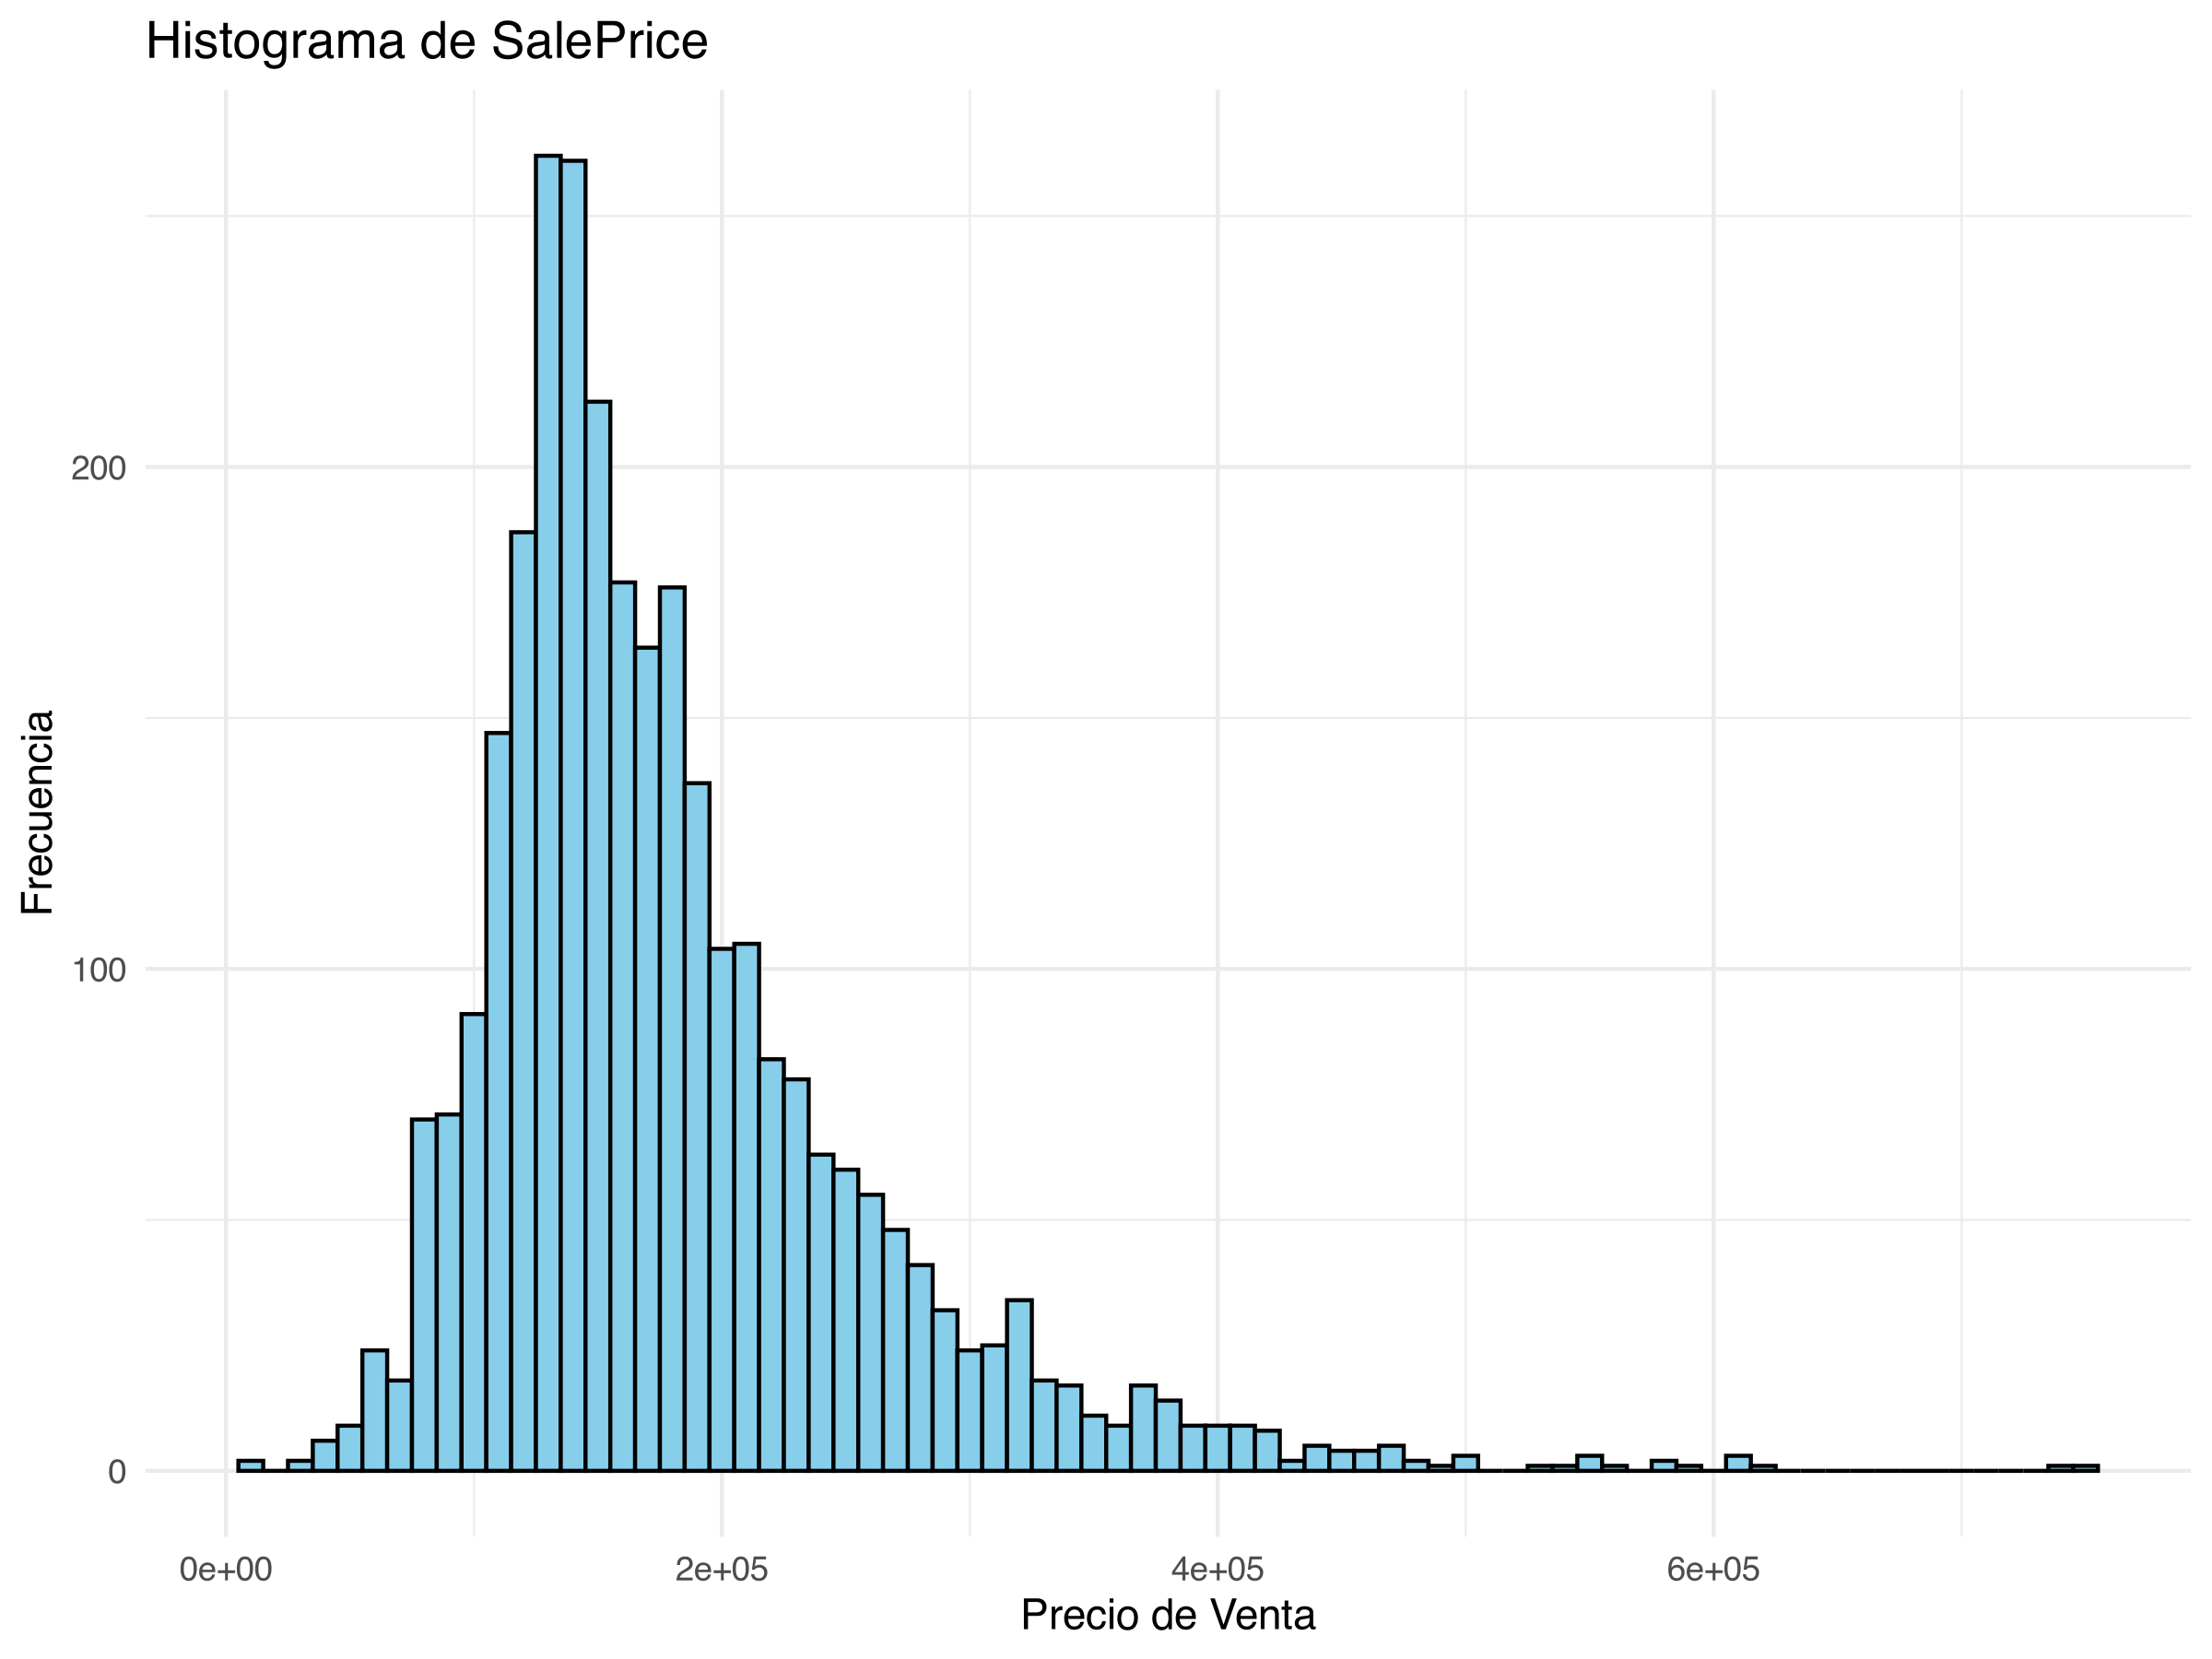
\includegraphics[width=0.8\textwidth]{images/histograma_saleprice.png}
    \caption{Histograma de la variable \textit{SalePrice}, mostrando la frecuencia de precios de venta. Se observa una clara asimetría positiva.}
    \label{fig:histograma}
\end{figure}

\begin{figure}[H]
    \centering
    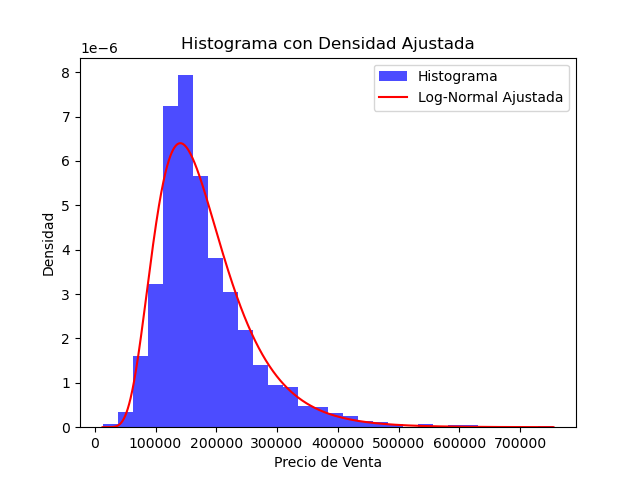
\includegraphics[width=0.8\textwidth]{images/densidad_ajustada.png}
    \caption{Histograma de \textit{SalePrice} con la densidad log-normal ajustada. La curva ajustada refleja la forma asimétrica positiva observada en los datos.}
    \label{fig:densidad_ajustada}
\end{figure}

\begin{figure}[H]
    \centering
    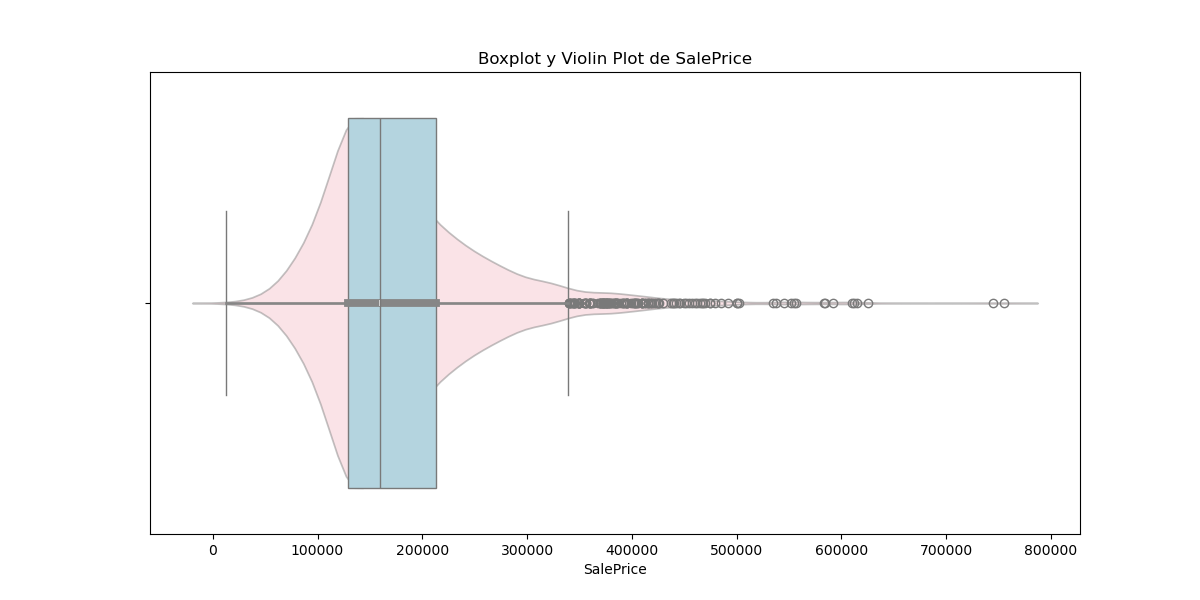
\includegraphics[width=0.8\textwidth]{images/boxplot_violin_saleprice.png}
    \caption{Boxplot y violin plot de la variable \textit{SalePrice}. El boxplot muestra valores atípicos en la cola superior, mientras que el violin plot destaca la densidad de precios alrededor de la mediana.}
    \label{fig:boxplot_violin}
\end{figure}


\subsection{Análisis de Resultados}

El análisis de los resultados obtenidos a través de las simulaciones y los ajustes realizados en los datos se complementa con los gráficos generados. Estos gráficos no solo proporcionan una representación visual de los datos, sino que también nos permiten identificar patrones, evaluar la precisión de los modelos ajustados y obtener conclusiones sobre la distribución de los precios de las casas en Ames, Iowa.

\subsubsection{Histograma de \textit{SalePrice} (Figura \ref{fig:histograma})}
El histograma de la variable \textit{SalePrice} muestra claramente la distribución de los precios de venta de las casas. Se observa una distribución con una asimetría positiva, lo que significa que la mayoría de los precios se agrupan en el rango inferior, mientras que hay un número reducido de casas con precios significativamente altos. Esta asimetría sugiere la presencia de una cola en la parte superior de la distribución, lo que es común en mercados inmobiliarios donde algunas propiedades de lujo o muy demandadas tienen precios mucho mayores que la mayoría de las casas.

\subsubsection{Ajuste de la Densidad Log-Normal (Figura \ref{fig:densidad_ajustada})}
En la segunda figura, se superpone el histograma de \textit{SalePrice} con la densidad log-normal ajustada. El ajuste de la distribución log-normal refleja bien la forma de la distribución observada, con una cola hacia la derecha que coincide con la asimetría positiva observada en el histograma. La curva ajustada se alinea de manera precisa con la distribución empírica de los datos, lo que sugiere que una distribución log-normal es un modelo adecuado para describir la variable \textit{SalePrice}. Esto valida la elección del modelo para realizar cálculos de probabilidades y estimaciones de valores esperados en el análisis posterior.

\subsubsection{Boxplot y Violin Plot (Figura \ref{fig:boxplot_violin})}
Los diagramas de caja (boxplot) y violín (violin plot) proporcionan una visión adicional sobre la dispersión de los precios de las casas y la presencia de valores atípicos. En el boxplot, se observa que la mediana de los precios está bastante alejada de la media, lo que es indicativo de la asimetría positiva mencionada anteriormente. Además, el boxplot muestra varios valores atípicos en la cola superior, lo que refuerza la idea de que existen casas con precios excepcionalmente altos. El violin plot, por su parte, proporciona una representación más detallada de la densidad de los precios, destacando la concentración de casas en el rango más bajo de precios y la disminución de la densidad a medida que los precios aumentan. Este gráfico también confirma la forma sesgada de la distribución, con una mayor concentración de precios cercanos a la mediana y menos casas en los rangos más altos.

\subsubsection{Conclusiones del Análisis}
En conjunto, los gráficos y los modelos ajustados ofrecen una comprensión detallada de la distribución de los precios de venta de casas en Ames, Iowa. La asimetría positiva observada en los datos es consistente con el modelo log-normal ajustado, que proporciona una descripción precisa de los datos. Además, la presencia de valores atípicos en el boxplot sugiere que algunas casas tienen precios significativamente más altos que el resto, lo que es un patrón común en muchos mercados inmobiliarios. Estos hallazgos permiten realizar inferencias sobre el comportamiento del mercado de viviendas en la región y proporcionan una base sólida para futuros análisis y decisiones basadas en probabilidades de precios.


\section{Conclusiones}

Este proyecto ha demostrado cómo los conceptos fundamentales de probabilidad y estadística pueden aplicarse eficazmente a una serie de problemas prácticos mediante el uso de herramientas computacionales y métodos de simulación. A través de la simulación Monte Carlo, hemos logrado abordar problemas complejos que no pueden resolverse fácilmente con métodos analíticos tradicionales, mostrando cómo la experimentación computacional puede proporcionar soluciones precisas y útiles en diversas situaciones.

Los principales hallazgos del proyecto incluyen:

\begin{itemize}
    \item En el \textbf{Problema 1}, se realizó un análisis detallado de los precios de las casas en Ames, Iowa. El uso de herramientas de visualización y el ajuste de una distribución log-normal permitieron modelar eficazmente los precios, y los cálculos de probabilidades y valores esperados proporcionaron información útil sobre el mercado inmobiliario local.
    
    \item En el \textbf{Problema 2}, se empleó la simulación de Monte Carlo para estimar la cantidad de asientos extra que una aerolínea podría vender, basándose en un modelo de no presentación de pasajeros. Este análisis reveló que es posible optimizar la venta de asientos, maximizando ingresos sin exceder la capacidad de los aviones.
    
    \item En el \textbf{Problema 3}, se utilizó la simulación para calcular la probabilidad de que un peaje atienda más de 500 autos en un día. Mediante distribuciones normales y exponenciales, se pudo estimar con alta precisión esta probabilidad, proporcionando una herramienta valiosa para la planificación de recursos en el peaje.
    
    \item En el \textbf{Problema 4}, se modelaron los tiempos de espera, cirugía y postoperatorio en una sala de operaciones utilizando distribuciones normales, exponenciales y uniformes. La simulación de Monte Carlo permitió estimar el número de pacientes que se pueden operar en un mes, lo que puede ser útil para optimizar la programación de cirugías y la asignación de recursos.
    
    \item En el \textbf{Problema 5}, se calculó la distancia esperada entre dos distribuciones normales estándar. Este cálculo, basado en propiedades fundamentales de las distribuciones normales, tiene aplicaciones en la comparación de modelos estadísticos y en la evaluación de la similitud entre distribuciones.
\end{itemize}

A lo largo del proyecto, se ha evidenciado que los métodos estadísticos, y en particular la simulación Monte Carlo, son herramientas poderosas para resolver problemas complejos y para obtener soluciones aproximadas cuando los métodos analíticos son difíciles de aplicar. Los resultados obtenidos no solo validan las técnicas empleadas, sino que también muestran cómo estas pueden ser adaptadas a otros contextos reales, como la optimización de procesos, la toma de decisiones en situaciones de incertidumbre y la mejora de sistemas operativos.

Sin embargo, también se han identificado áreas de mejora y oportunidades para futuras investigaciones. En algunos casos, la precisión de los resultados podría mejorarse con un mayor número de simulaciones o mediante el ajuste de los modelos probabilísticos a datos más específicos. Además, la extensión de los métodos empleados a otros tipos de distribuciones o sistemas más complejos podría ofrecer nuevos insights en problemas similares.

En resumen, este proyecto ha permitido aplicar de manera efectiva técnicas avanzadas de probabilidad y estadística para resolver problemas reales. Los métodos de simulación, combinados con el análisis teórico, han demostrado ser altamente efectivos en la obtención de resultados útiles y aplicables a una amplia variedad de situaciones prácticas, desde el análisis económico hasta la optimización de procesos operativos.


\section{Apéndices}
\subsection{Código Fuente}
\href{https://github.com/Karimtek/MAT043-PRO}{Repositorio con código fuente}


\subsection{Referencias}

\href{https://www.youtube.com/playlist?list=PLRdsr8w_wLNzYYSYP6bvf1p30mo27X9q-}{Playlist "Probabilidad y Estadística" por Profesor Ronny Vallejos}

\end{document}
